
\chapter{Experimental Results and Analysis}
\section{Overall Model Performance}
All three classifiers are evaluated using the same held-out test set of 2,947 observations. Table~\ref{tab:overall} summarises the results. \emph{Random Forest achieves the highest accuracy (92.87\%), macro precision (93.00\%), macro recall (92.58\%) and macro F1-score (92.70\%).} KNN ranks second in accuracy, while Decision Tree gives the lowest overall scores among the three evaluated models.


\begin{table}[H]\centering
\caption{Overall test-set performance comparison}\label{tab:overall}
\begin{tabular}{lrrrr}
\toprule
\textbf{Model} & \textbf{Accuracy} & \textbf{Macro precision} & \textbf{Macro recall} & \textbf{Macro F1}\\
\midrule
KNN & 88.02\% & 88.97\% & 87.46\% & 87.66\% \\
Decision Tree & 86.22\% & 86.25\% & 85.87\% & 85.95\% \\
Random Forest & 92.87\% & 93.00\% & 92.58\% & 92.70\% \\
\bottomrule
\end{tabular}
\end{table}

\section{Model Comparison Graph}
Figure~\ref{fig:modelcomp} compares accuracy and macro F1-score. Both measures show the same ranking: Random Forest, KNN and Decision Tree. The gap between Random Forest and KNN is approximately 4.85 percentage points in accuracy, while the gap between Random Forest and Decision Tree is approximately 6.65 percentage points.

\begin{figure}[H]\centering
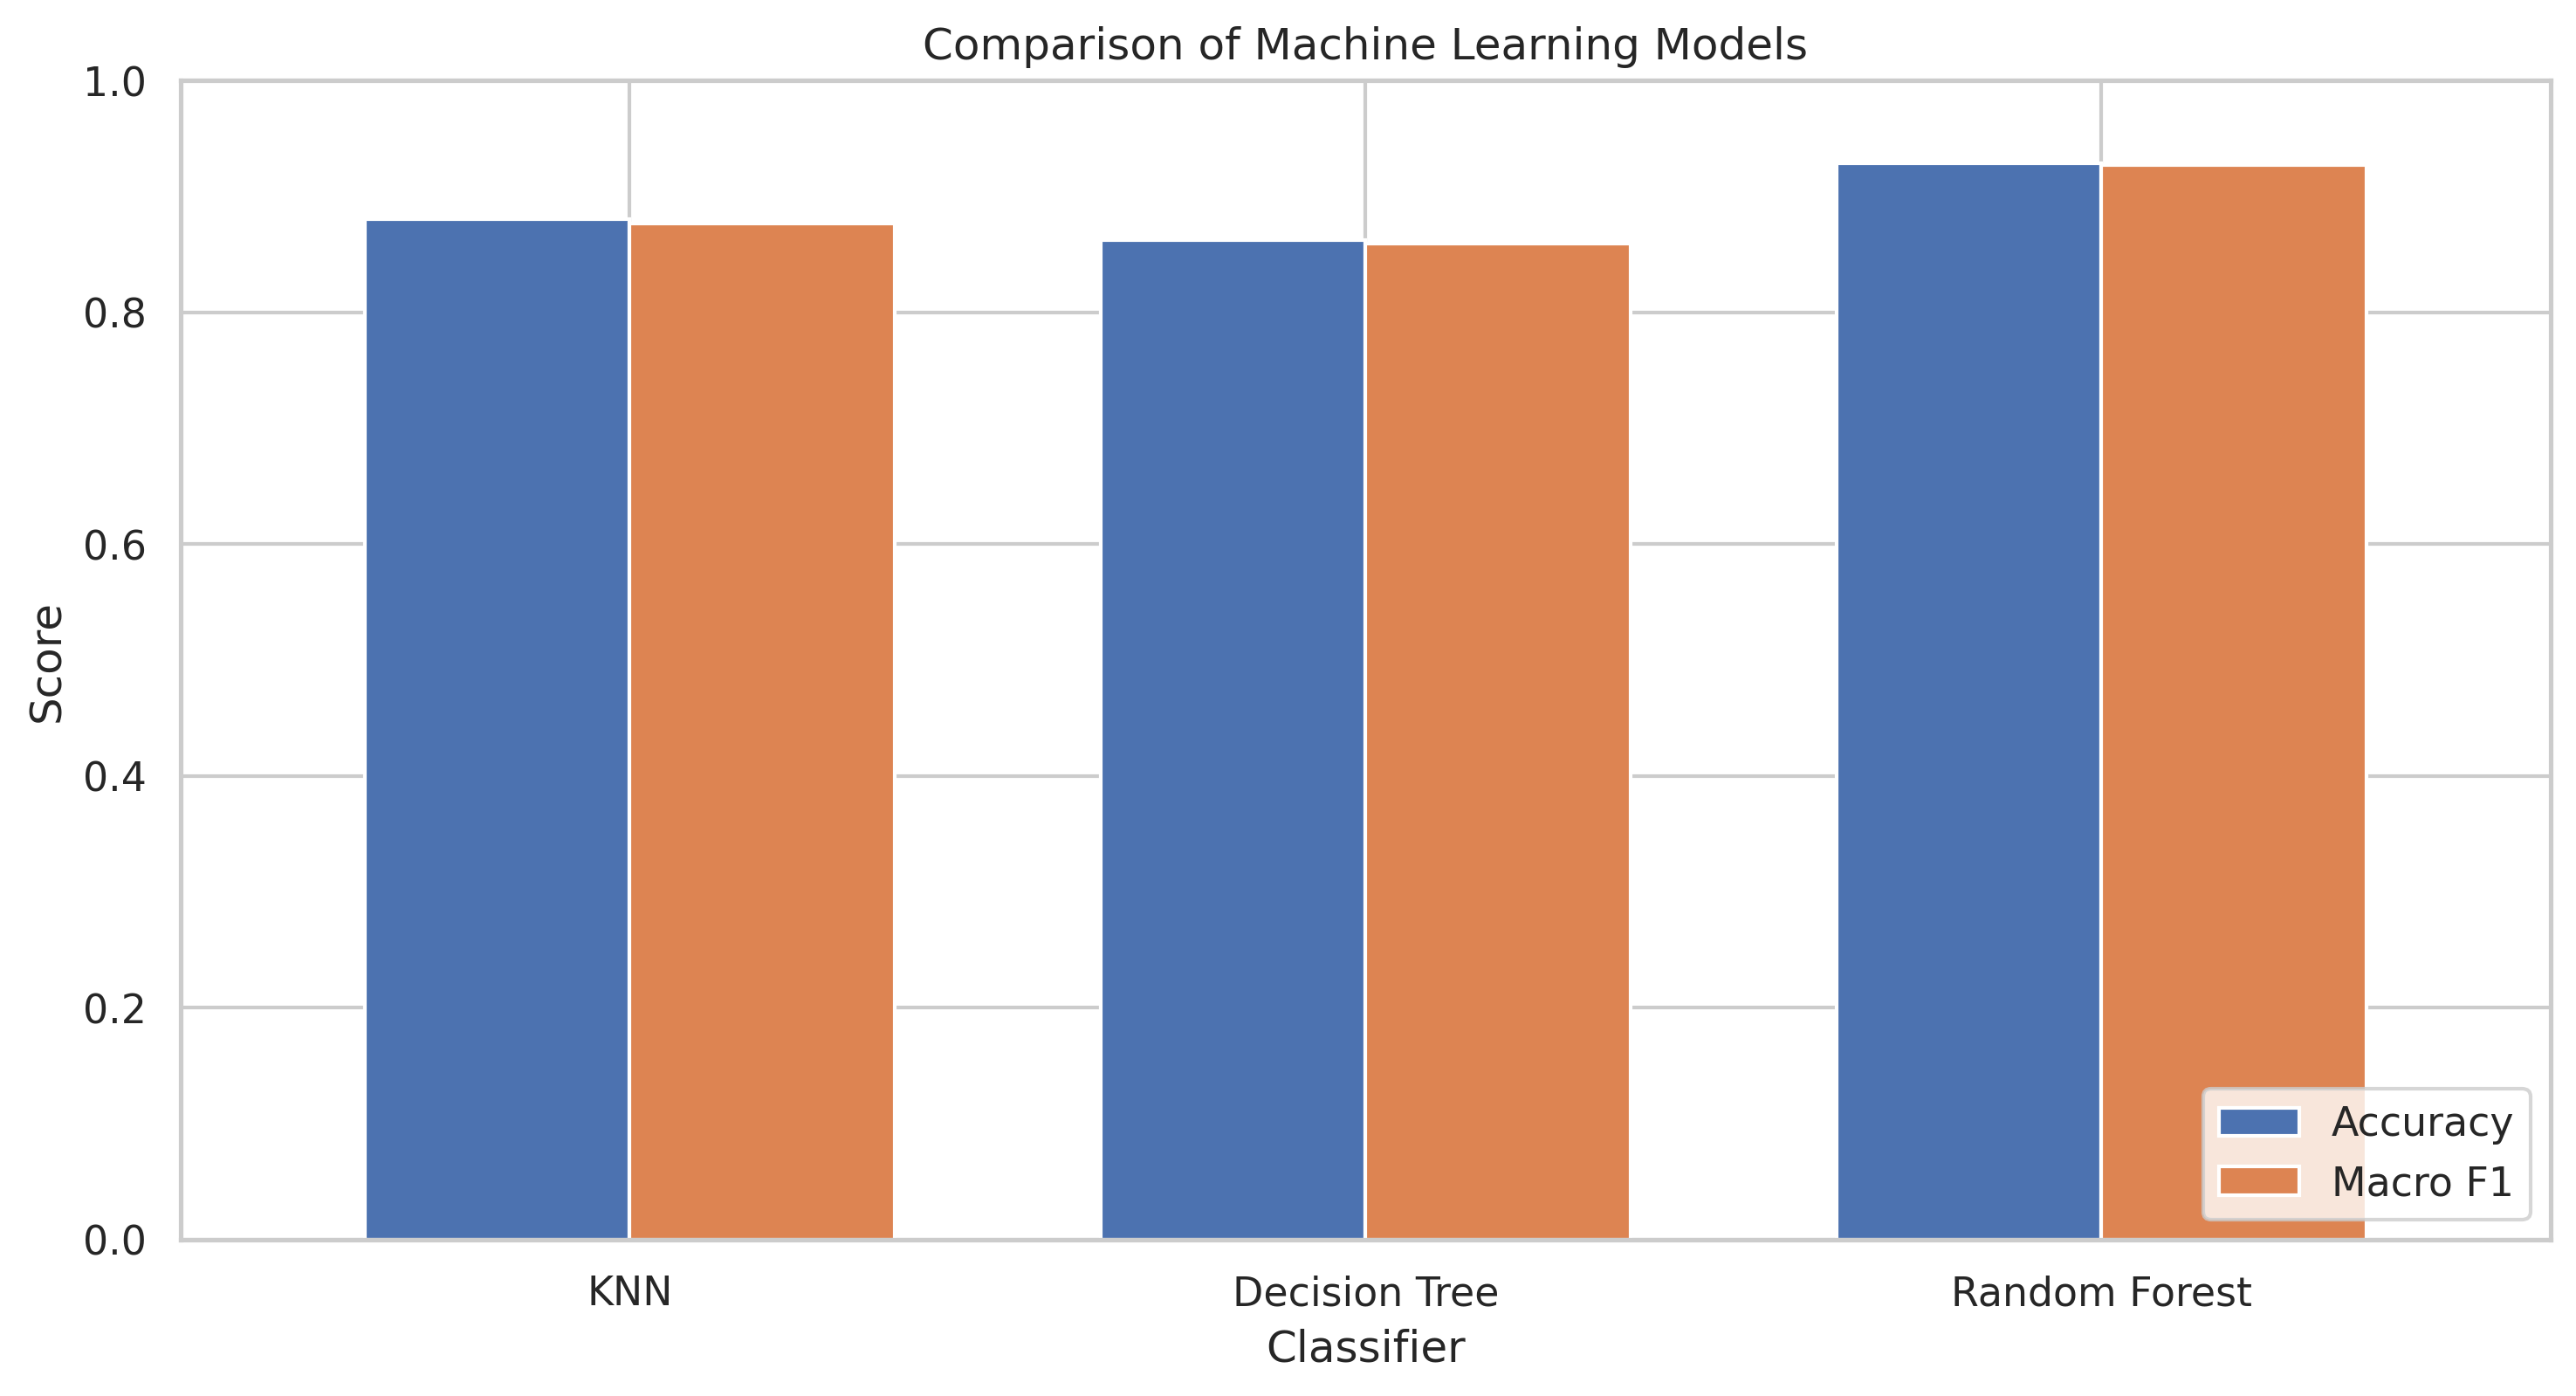
\includegraphics[width=0.9\textwidth]{model_comparison.png}
\caption{Accuracy and macro F1-score comparison.}
\label{fig:modelcomp}
\end{figure}

\section{Confusion Matrix Analysis}
A confusion matrix compares actual class labels with predicted class labels. Correct predictions appear along the main diagonal, while off-diagonal values represent misclassifications. The row labels in the following figures correspond to actual activities and the column labels correspond to predicted activities.

\begin{figure}[H]\centering
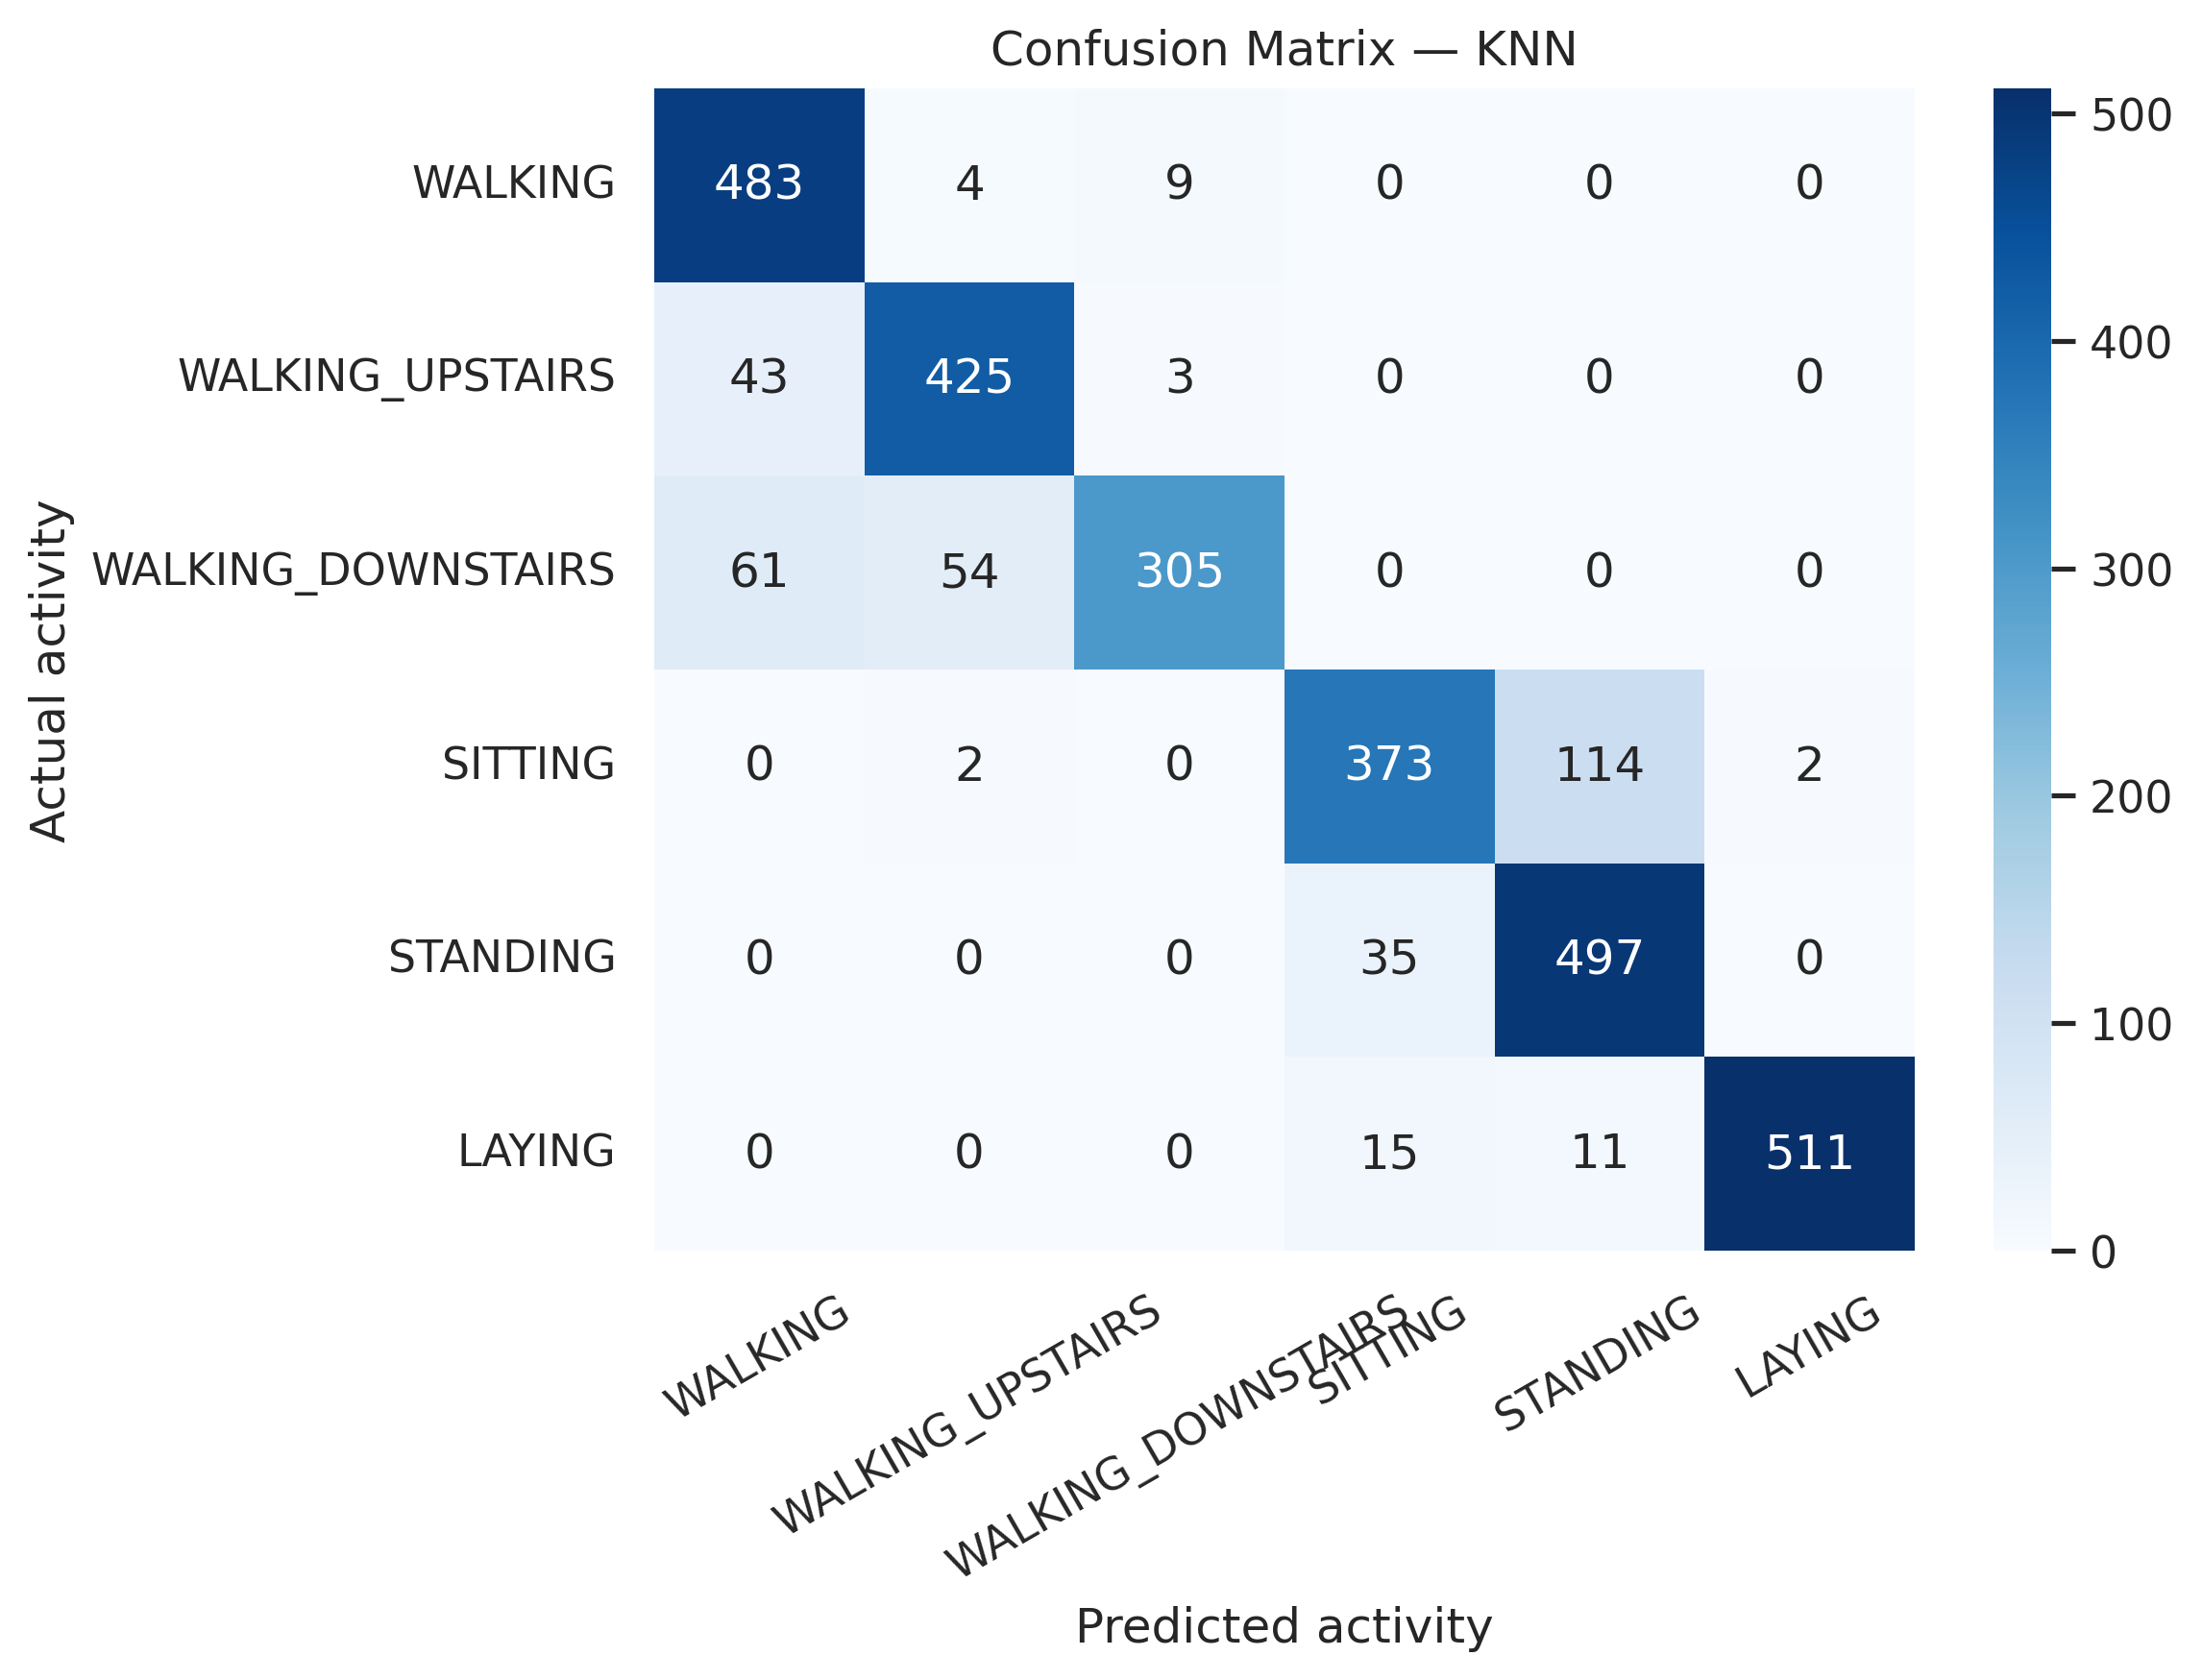
\includegraphics[width=0.88\textwidth]{confusion_knn.png}
\caption{Confusion matrix for KNN.}
\label{fig:cmknn}
\end{figure}
For KNN, the model correctly identifies 483 of 496 walking observations and 511 of 537 laying observations. A notable confusion occurs between walking downstairs and walking: 61 walking-downstairs observations are predicted as walking. Sitting and standing are also confused in both directions.

\begin{figure}[H]\centering
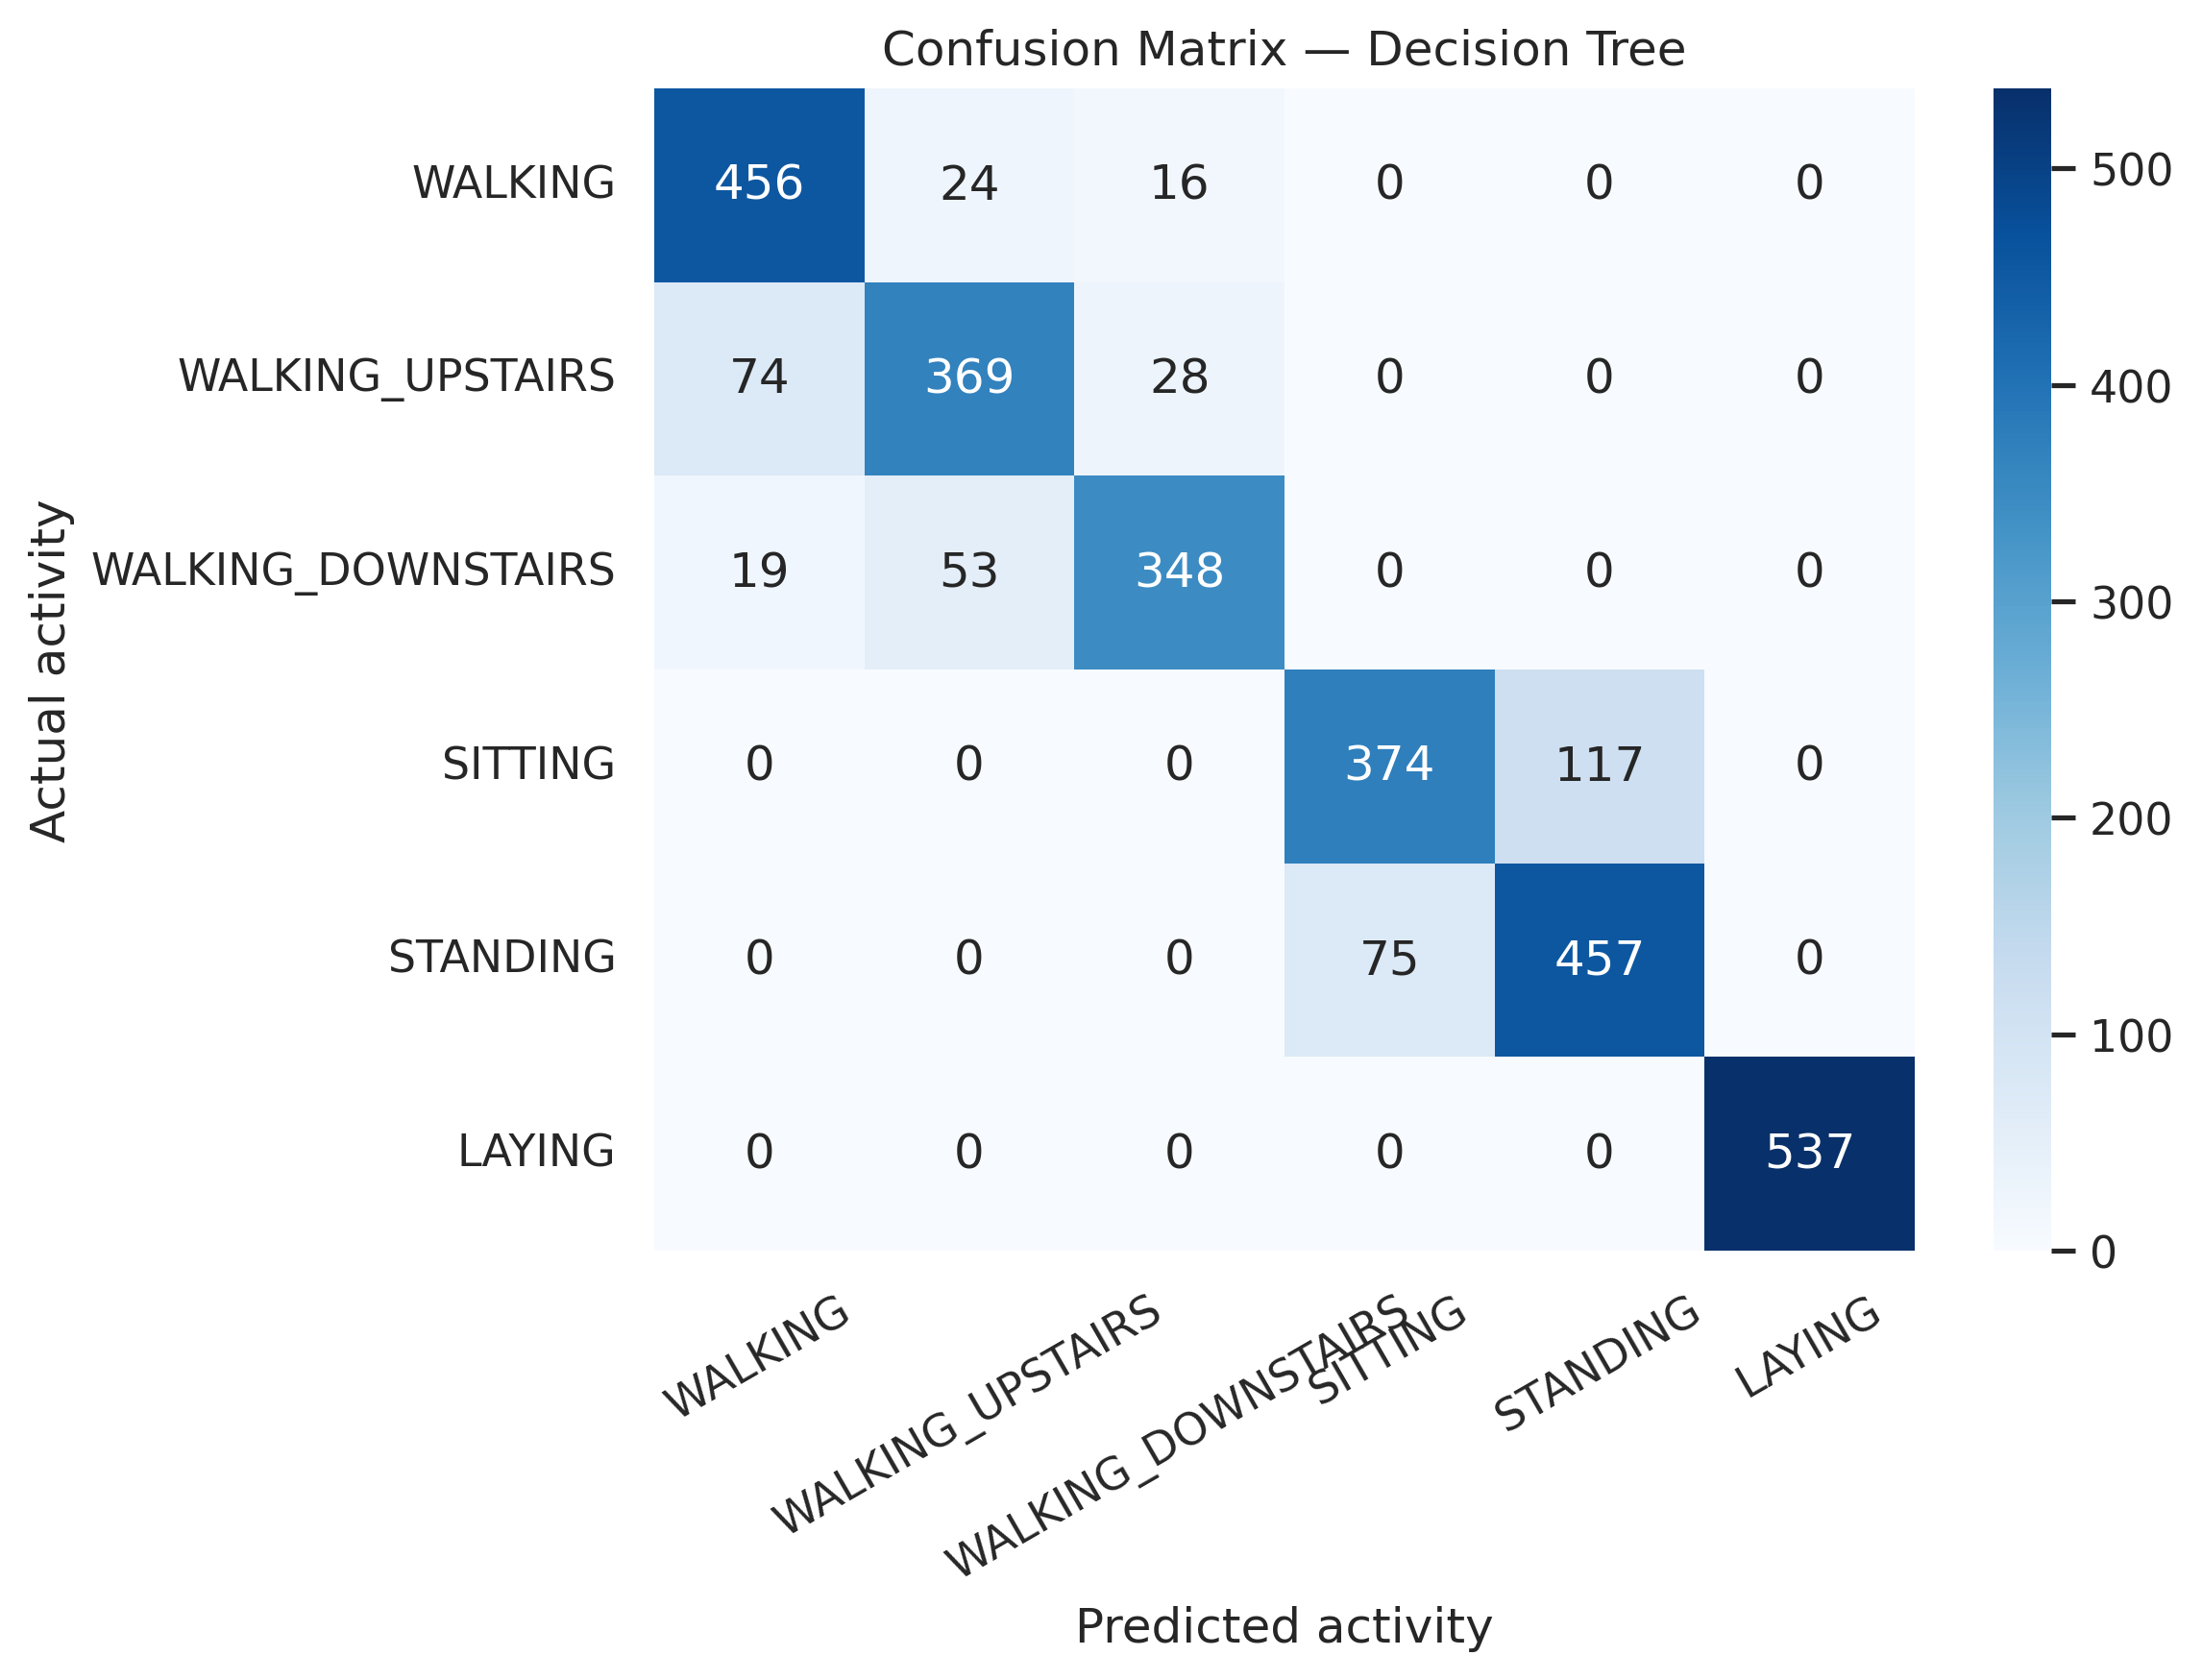
\includegraphics[width=0.88\textwidth]{confusion_decision_tree.png}
\caption{Confusion matrix for Decision Tree.}
\label{fig:cmdt}
\end{figure}
The Decision Tree correctly classifies all 537 laying test observations. However, it confuses sitting with standing: 117 sitting observations are predicted as standing, and 75 standing observations are predicted as sitting. Some confusion is also present among the three walking-related classes.

\begin{figure}[H]\centering
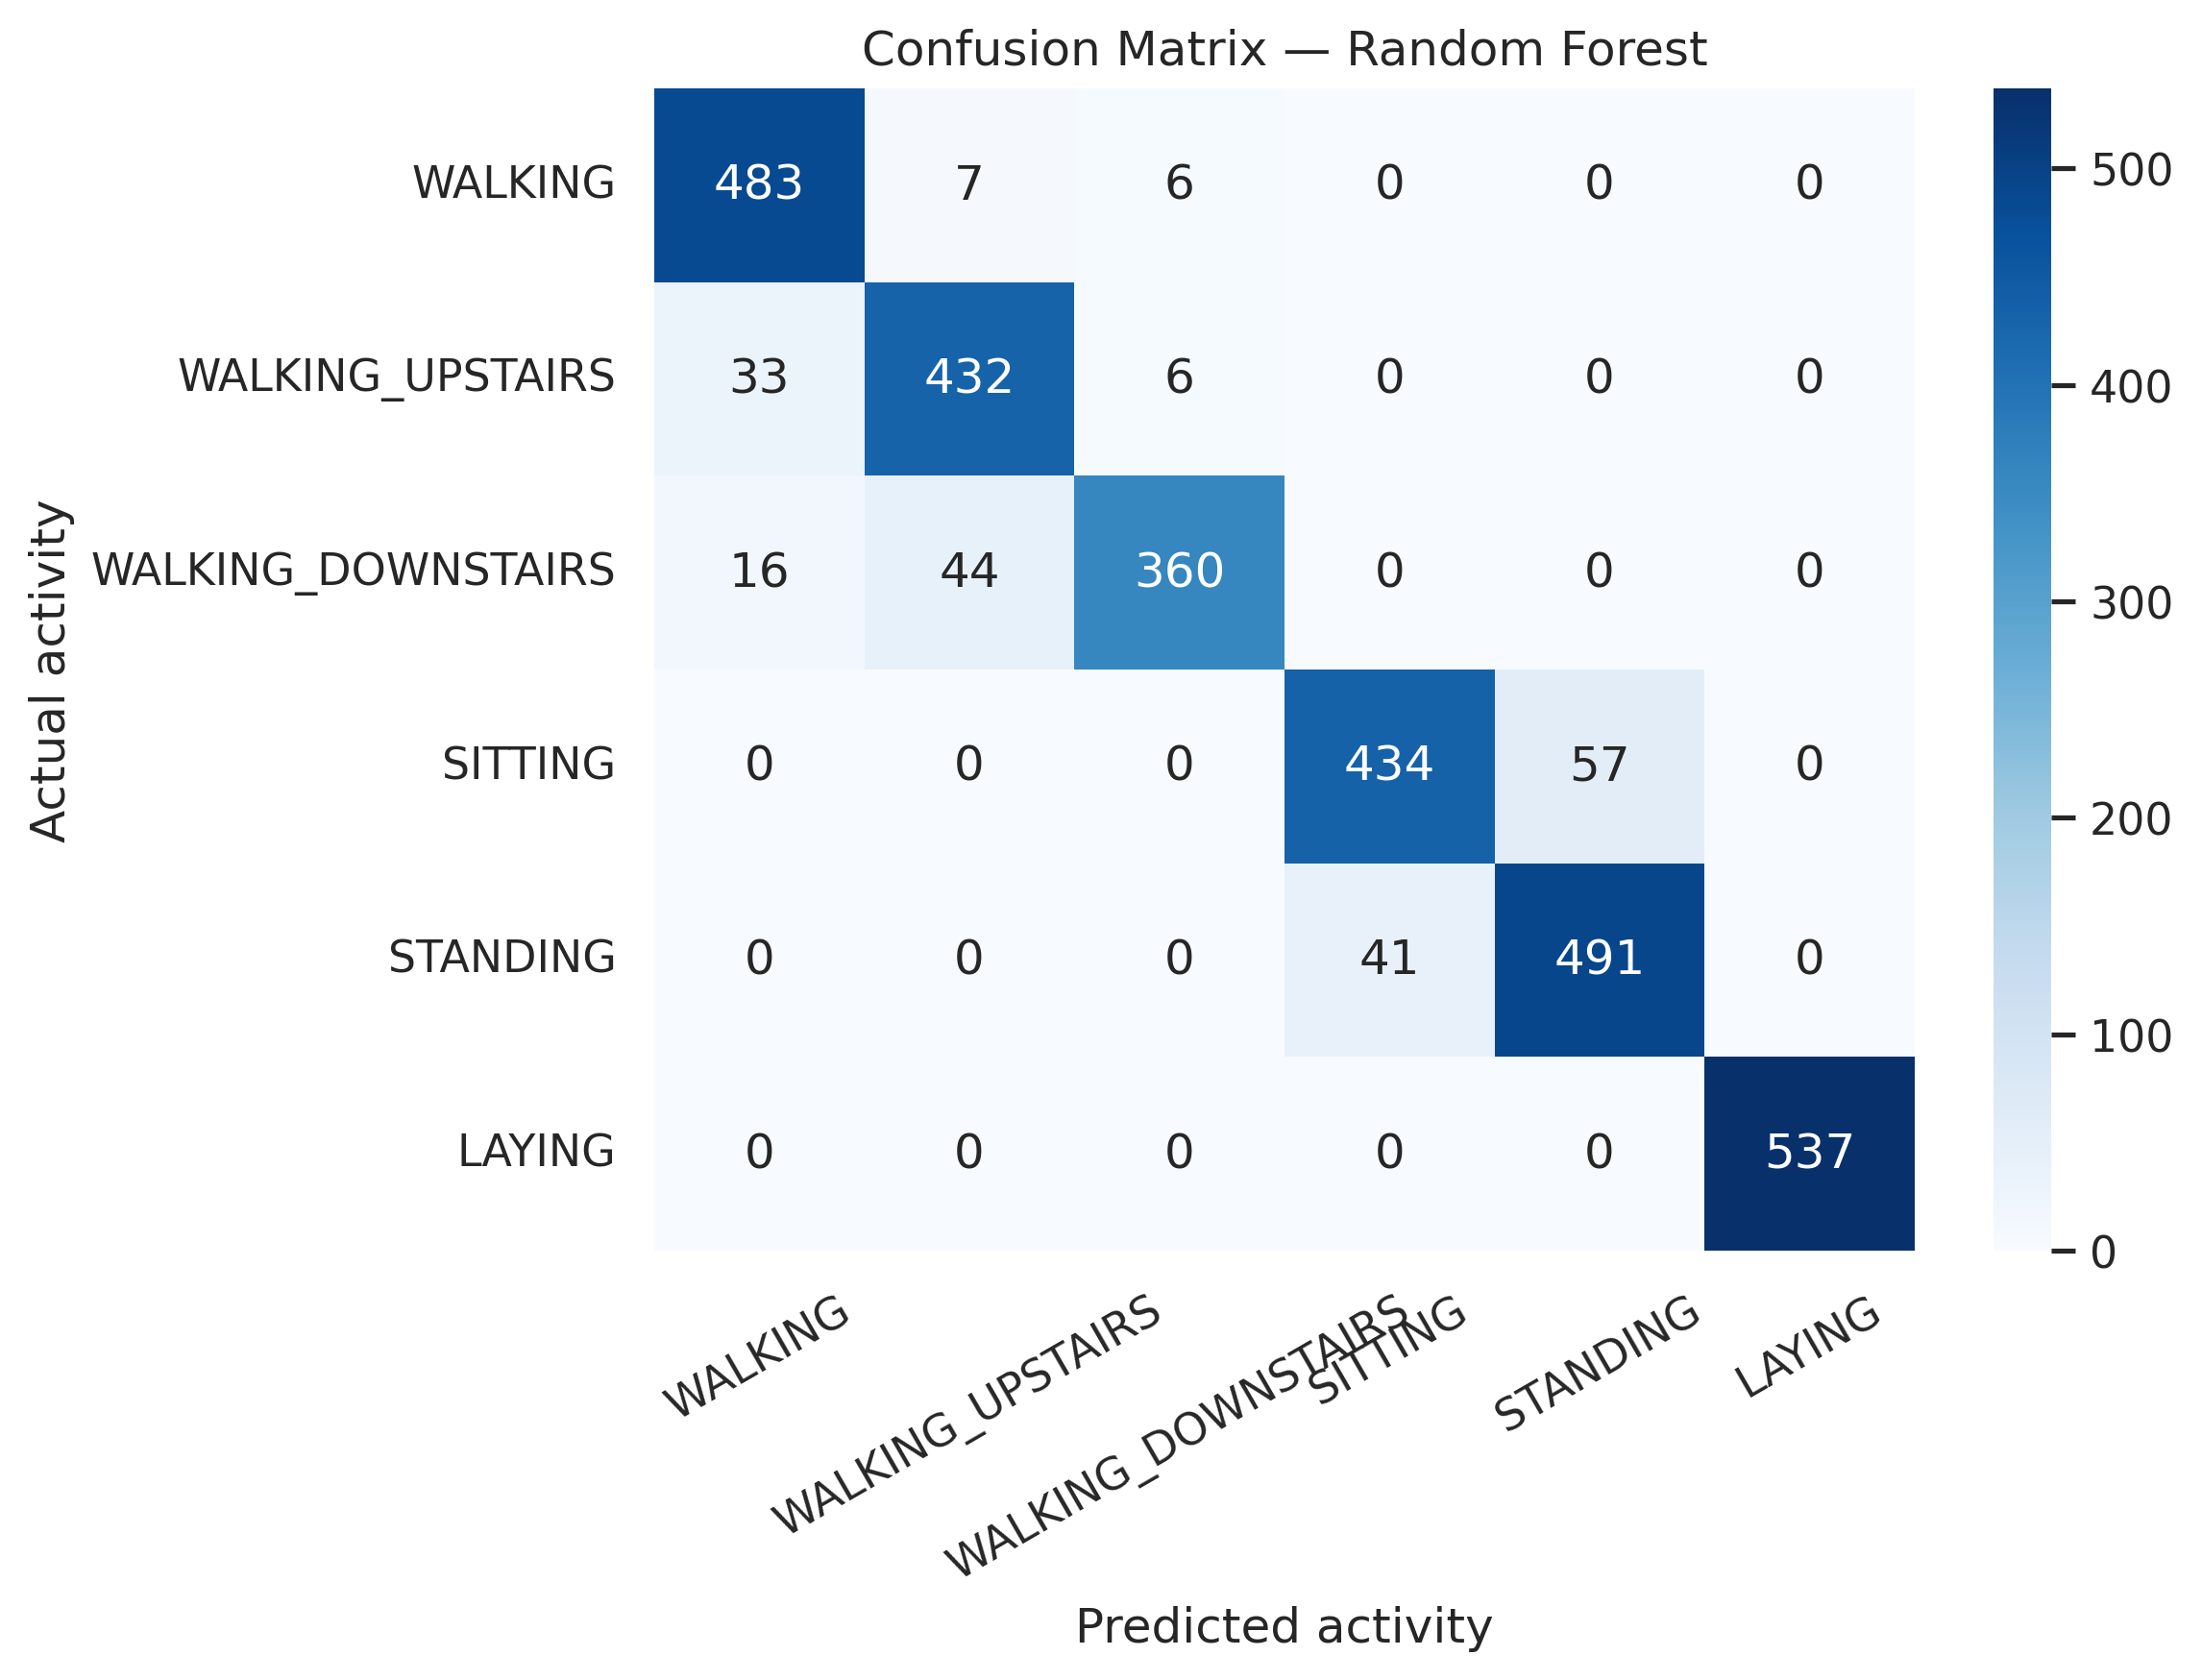
\includegraphics[width=0.88\textwidth]{confusion_random_forest.png}
\caption{Confusion matrix for Random Forest.}
\label{fig:cmrf}
\end{figure}
Random Forest correctly classifies all 537 laying observations. It also improves the separation of sitting and standing compared with the other two models, although 57 sitting observations are predicted as standing and 41 standing observations are predicted as sitting. Among dynamic activities, the main remaining confusion is between walking and walking downstairs.

\section{Class-wise Evaluation}
The following tables provide class-wise precision, recall, F1-score and support. Support is the number of actual test observations belonging to the corresponding class. These tables provide more detail than overall accuracy alone.

\subsection{Class-wise report: KNN}
\begin{table}[H]\centering
\caption{Class-wise precision, recall and F1-score for KNN}
\begin{tabular}{lrrrr}
\toprule
\textbf{Activity} & \textbf{Precision} & \textbf{Recall} & \textbf{F1-score} & \textbf{Support}\\
\midrule
WALKING & 0.823 & 0.974 & 0.892 & 496 \\
WALKING\_UPSTAIRS & 0.876 & 0.902 & 0.889 & 471 \\
WALKING\_DOWNSTAIRS & 0.962 & 0.726 & 0.828 & 420 \\
SITTING & 0.882 & 0.760 & 0.816 & 491 \\
STANDING & 0.799 & 0.934 & 0.861 & 532 \\
LAYING & 0.996 & 0.952 & 0.973 & 537 \\
\bottomrule
\end{tabular}
\end{table}

\subsection{Class-wise report: Decision Tree}
\begin{table}[H]\centering
\caption{Class-wise precision, recall and F1-score for Decision Tree}
\begin{tabular}{lrrrr}
\toprule
\textbf{Activity} & \textbf{Precision} & \textbf{Recall} & \textbf{F1-score} & \textbf{Support}\\
\midrule
WALKING & 0.831 & 0.919 & 0.873 & 496 \\
WALKING\_UPSTAIRS & 0.827 & 0.783 & 0.805 & 471 \\
WALKING\_DOWNSTAIRS & 0.888 & 0.829 & 0.857 & 420 \\
SITTING & 0.833 & 0.762 & 0.796 & 491 \\
STANDING & 0.796 & 0.859 & 0.826 & 532 \\
LAYING & 1.000 & 1.000 & 1.000 & 537 \\
\bottomrule
\end{tabular}
\end{table}

\subsection{Class-wise report: Random Forest}
\begin{table}[H]\centering
\caption{Class-wise precision, recall and F1-score for Random Forest}
\begin{tabular}{lrrrr}
\toprule
\textbf{Activity} & \textbf{Precision} & \textbf{Recall} & \textbf{F1-score} & \textbf{Support}\\
\midrule
WALKING & 0.908 & 0.974 & 0.940 & 496 \\
WALKING\_UPSTAIRS & 0.894 & 0.917 & 0.906 & 471 \\
WALKING\_DOWNSTAIRS & 0.968 & 0.857 & 0.909 & 420 \\
SITTING & 0.914 & 0.884 & 0.899 & 491 \\
STANDING & 0.896 & 0.923 & 0.909 & 532 \\
LAYING & 1.000 & 1.000 & 1.000 & 537 \\
\bottomrule
\end{tabular}
\end{table}

\section{Feature Importance}
Random Forest provides an estimate of the relative importance of input features. Figure~\ref{fig:importance} shows the 20 features with the highest importance scores in the fitted model. The most important feature is \texttt{tGravityAcc-mean()-X}, with an importance score of approximately 0.03850. Other highly ranked features include gravity acceleration statistics and angle-related features.

\begin{figure}[H]\centering
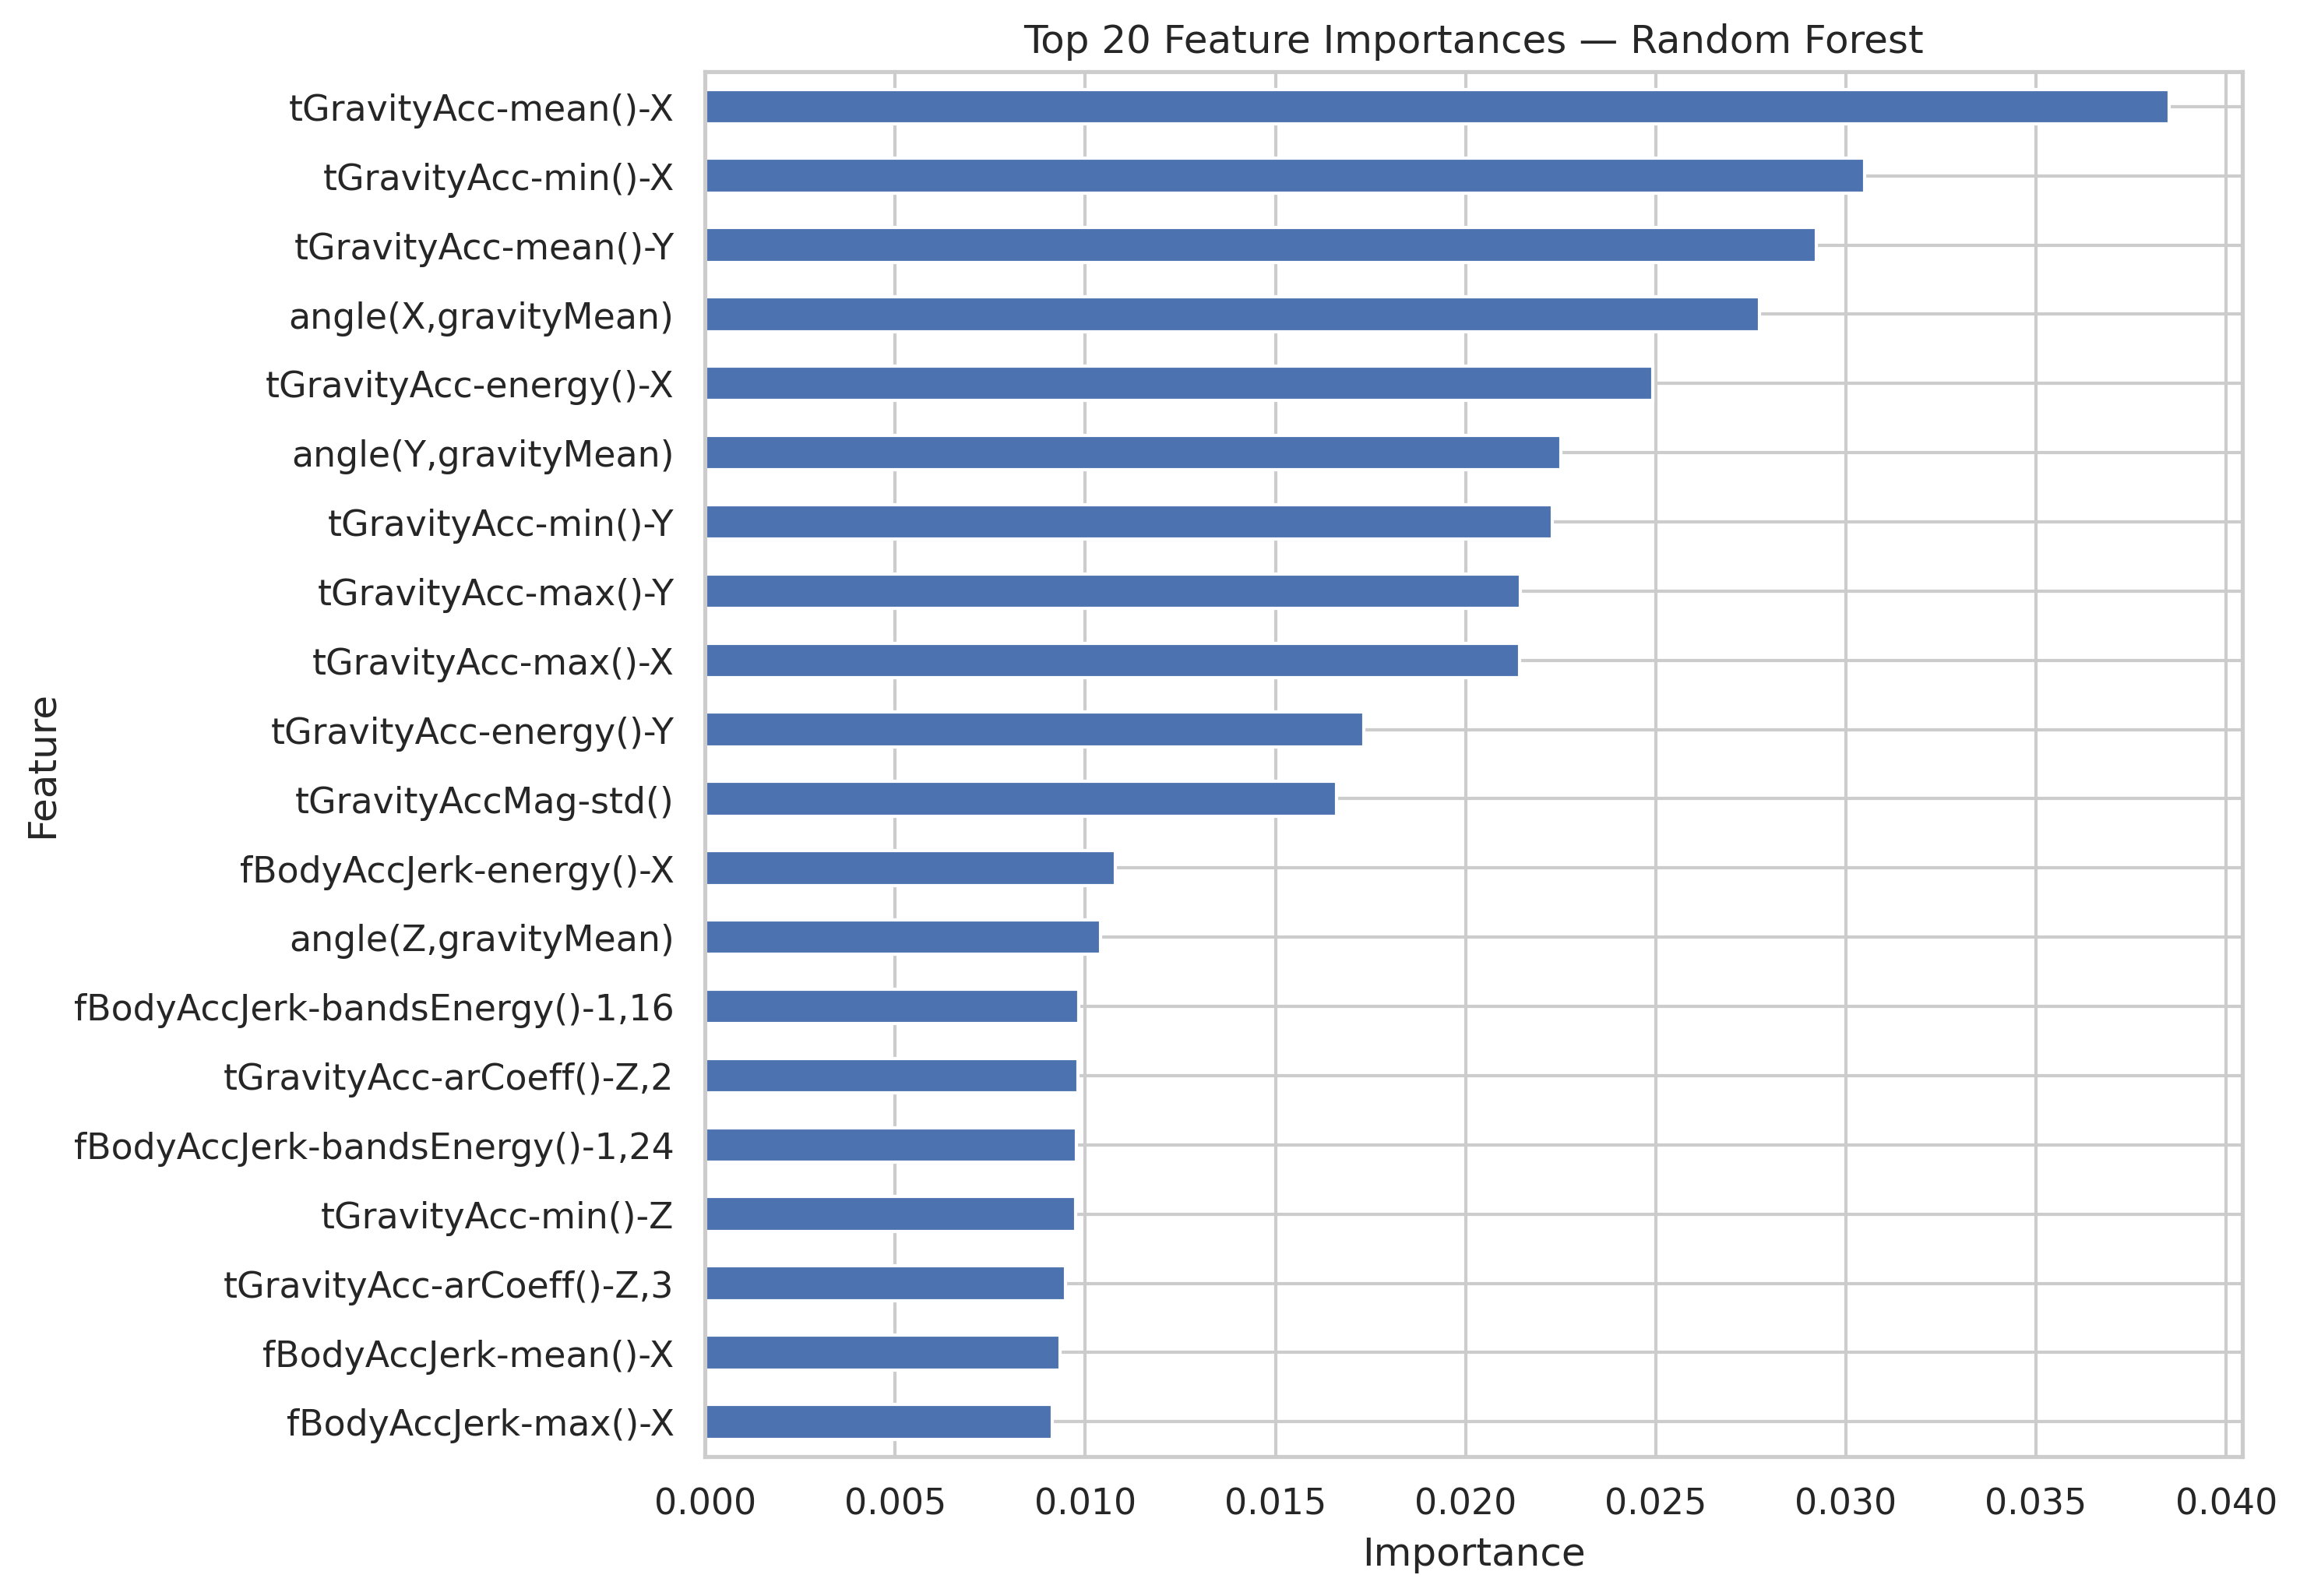
\includegraphics[width=0.95\textwidth]{feature_importance_top20.png}
\caption{Top 20 features ranked by Random Forest feature importance.}
\label{fig:importance}
\end{figure}

\begin{table}[H]\centering
\caption{Top 10 Random Forest features by importance}
\begin{tabular}{lr}
\toprule
\textbf{Feature} & \textbf{Importance}\\
\midrule
tGravityAcc-mean()-X & 0.03850 \\
tGravityAcc-min()-X & 0.03048 \\
tGravityAcc-mean()-Y & 0.02923 \\
angle(X,gravityMean) & 0.02773 \\
tGravityAcc-energy()-X & 0.02492 \\
angle(Y,gravityMean) & 0.02251 \\
tGravityAcc-min()-Y & 0.02228 \\
tGravityAcc-max()-Y & 0.02144 \\
tGravityAcc-max()-X & 0.02143 \\
tGravityAcc-energy()-Y & 0.01733 \\
\bottomrule
\end{tabular}
\end{table}

Feature importance indicates which variables contributed most to the fitted forest's decisions. It does not by itself establish a causal relationship between a sensor feature and a physical activity.

\section{Single-Observation Prediction}
The notebook demonstrates prediction for one test observation (sample index 0) using the Random Forest classifier. The actual activity is \textbf{STANDING}, and the predicted activity is also \textbf{STANDING}. This example demonstrates the inference call for one feature vector.

\section{Best Model}
\emph{Random Forest is selected as the best model because it achieves the highest macro F1-score (0.9270) and highest accuracy (0.9287) among the evaluated classifiers.} It is therefore the model selected for the best-performing result in this experiment.
